\documentclass[twocolumn,a4paper,13pt]{book}
\usepackage{booktabs,chemformula}
\setcounter{page}{108}
\usepackage{caption}
\usepackage{graphicx}

\captionsetup{labelformat=empty}
\begin{document}	
	\begin{table}[h!]
	\textbf{table 6.8 Software Problem Severity Levels}
		\begin{tabular}{|p{1.5cm}|p{5.5cm}|}
			\toprule
			\textbf{severity}  & \textbf{Severity Level if the Problem}\\
			\midrule
			\ch{1} & Adversely affects the accomplishment of an
			“essential” system capability and there is no
			feasible workaround solution. —or—
			Adversely affects the technical, cost, or
			schedule risks to the project, or to its life
			cycle support system, and there is no feasible
			workaround solution available \\
			\hline\ch{2} & Can seriously impact any requirement
			identifed as “critical” —or—
			Prevents the accomplishment of an
			“essential” system capability \\
			\hline\ch{3} &Adversely affects the accomplishment of an
			“essential” system capability but there is a
			feasible workaround solution. —or—
			Adversely affects the technical, cost, or
			schedule risks to the project, or to its life
			cycle support system, but there is a feasible
			workaround solution available \\
			\hline\ch{4} & Is an inconvenience or annoyance to the
			system users/operators but does not affect a
			required operational or system essential
			capability. —or—
			Is an inconvenience or annoyance for
			development or maintenance personnel, but
			does not interfere with accomplishment of
			their responsibilities \\
			\hline \ch{5} & Has little or no impact and does not match
			description of severity levels 1–4 \\
			\bottomrule
		\end{tabular}
		
	\end{table}
evidence that the process is being followed. Process audit
Corrective Action requests should be retained by SQA.
Corrective Action measurements must also be collected
including SCRs/SDRs opened, closed and deferred; and
aging metrics for SCRs/SDRs open for 30, 60, and 90 days,
plus root cause. SCM is usually responsible for control and
status updating of the SCR/SDR databases and overseeing
the change management process. All SCRs/SDRs should be
retained by SCM through the end of the contract.\\
\textbf{6.4.3 Confguration Control Boards}
On large programs, there is typically a hierarchy of
Confguration Control Boards with different levels of control and responsibilities. On smaller programs, there is less
formality; however, some group(s) must exist to review and
approve changes and resolve conflicts like an Engineering
Review Board or a “Tiger Team.” Figure 6.7 is an example of
the typical relationship of CCBs.
Software CM supports all of the change boards depicted
in the example shown in Figure 6.7. At the very top of the hierarchy is the customer’s technical support CCB (or
Program Ofce CCB). Tey participate in, and monitor, the
activities of the lower level CCBs as needed.
The program level boards include the Confguration
Control Board (Program CCB) and the Software
Confguration Control Board (Sw/CCB). At the subsystem
level, there may be three lower level boards: the Subsystem
Confguration Control Board (Subsystem CCB), the
Software CCB, and the Engineering Review Board. The suppliers (subcontractors) may also have similar levels of control
boards and, as the Software Project Manager, you should
have cognizance of the effectiveness of their boards.
Problems or issues for Software Units (SUs) with only
subsystem internal changes should be handled with SCRs/
SDRs by the subsystem’s control board. Baselined software with external subsystem interface changes must be
handled with SCRs/SDRs by the program-level Software
Confguration Control Board (Sw/CCB) or the program-level
CCB. Problems or issues for SIs with no interfaces should be
handled with SCRs/SDRs by the respective subsystem’s control board. The program-level Sw/CCB also has cognizance
over the Product Development Baseline.
The Responsible Software Engineer (RSE), usually one
of the Software Leads, provides support to the subsystem
boards. All of these boards must be described in the SDP or
the SCMP. The functions and relationships of the fve typical
CCBs are briefly described below:
- Program Confguration Control Board: The Program
CCB operates under the authority of the customer’s
CCB and approves changes to baselined documents
that affect cost, schedule, program constraints or
scope issues. Tere may also be a high-level Program
Confguration Evaluation Board (CEB). The CCB has
cognizance over Allocated and Product Baselines.
 Software Confguration Control Board: The Sw/CCB
operates under the authority of the Program CCB; it
has control over software changes at the system and
subsystem-to-subsystem 
%\begin{strip}
%	\centering
%	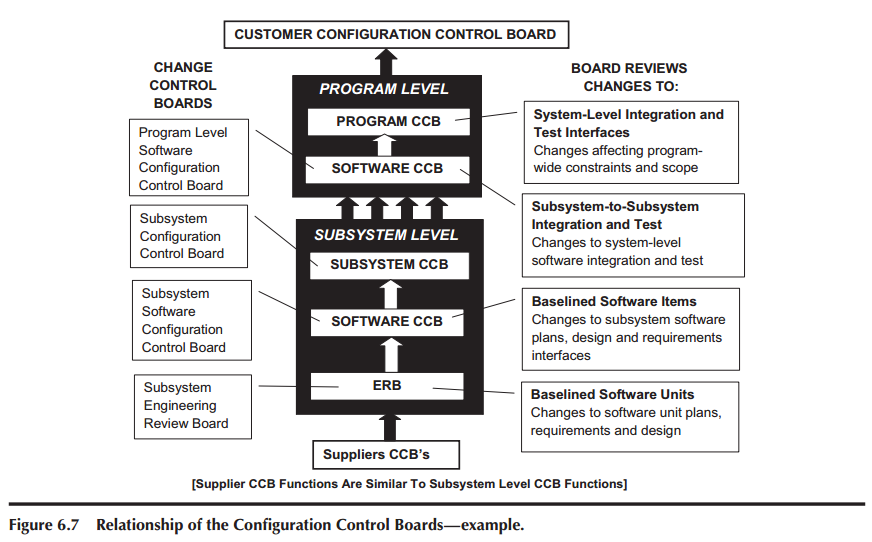
\includegraphics{ccb.png}	
%\end{strip}
software integration and test
level. The Sw /CCB has cognizance over the Product
Development Baseline for software, the Master
Software Development Library, and software risk
management.
- Subsystem Change Control Board: The subsystem CCB
must have control over changes found in baselined SIs.
It reviews SCRs/SDRs, provides impact assessments,
assigns appropriate personnel, and oversees the resolution and verifcation. The subsystem CCB must have
cognizance over the subsystem’s Allocated and Product
Development Baselines as well as the subsystem’s
Software Development Library.\\
- Subsystem Software Confguration Control Board:
Tis subsystem board reviews changes to baselined
SIs including changes to subsystem software plans,
designs, and requirements interfaces.
\begin{figure}[h!]
	\centering
	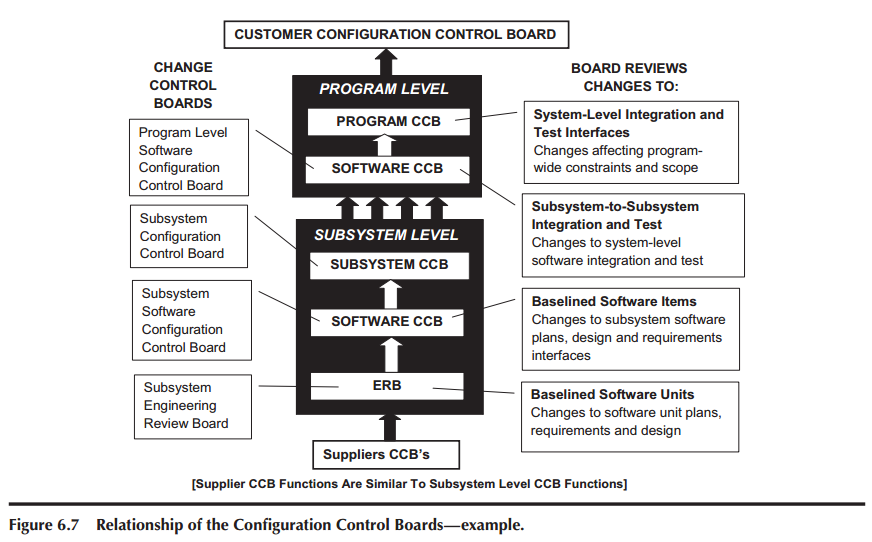
\includegraphics[width=0.5\textwidth]{ccb}
\end{figure}\\
- Engineering Review Board: Tis lower level board performs the same type of functions as the Subsystem
Software CCB but only controls changes found in
baselined SUs. Tis function can take place at the subsystem or at a lower level.\\
\textbf{Integration of the Corrective Action Process.} The
Corrective Action Process must be integrated across disciplines (Software, Hardware, Systems Engineering), all SwIPTs,
the Developer organizations (prime and suppliers), and the
System Development Life Cycle activities (from requirements defnition through System Test). In addition, the Corrective Action Process must be integrated with the risk management, Confguration Management, and the process improvement
processes. For example, risks, and risk mitigation actions, can become problems that need Corrective Action.\\
\textbf{6.4.4 When You Need a Paradigm Shift}\\ If you collect all of the relevant information available, you thoroughly analyze it, and you make the best-informed judgments and decisions for your project as to the best course of action, you did your job. However, sometimes the decisions you make are wrong, and the problems they create do not become apparent until well into the project. Do not be afraid to admit you made a mistake.
Instead, take Corrective Action as soon as you can to
revise the action plan and redirect the team. It will do great harm to your project if you fail to change course by being rigid and bull-headed. In this circumstance, you must implement a paradigm shift—a change to a new set of rules.
The characteristics and evolution of paradigms are well
covered by Barker (1998). As a futurist, Barker makes sense of what is happening in the business world. Understanding the paradigm shift concept is a frst step of trying to influence or control the future—of both your organization and your project. If you are not getting the expected results, fnd out why and make the needed changes to your project, regardless of how drastic or painful it may seem, before it is too late to affect the outcome.
Tese comments about the need to make paradigm shifts are
applicable to decisions made by your Board of Directors down to the workbench level. For example, IBM had a good business model with computer mainframes until Apple came along with laptops that forced IBM to apply the new paradigm in order to play the new game. Kodak was a leader in their industry until digital cameras came along and, since Kodak was apparently guilty of “paradigm paralysis,” they had to declare bankruptcy.\\\textbf{Contingency Planning.} Contingency planning is an element of change management but is often not included in the normal planning process. Tat is because it really is part of the post-planning process. In other words, after you and the team create the best possible plan, and associated planning documents, you should spend some time focused on contingency planning. Tis is often called “what-if” analysis. Pre-planning of this type can be very useful when things just don’t go the way you expected.\\\textbf{Lessons Learned.}If you don’t already know
this, you will fnd out that “things” have a way
of not going the way you expect them to. Most
of the time, contingency planning does not take
place until unfolding events requires you to do
it, but having alternate contingency plans in your
back pocket can be very helpful in time of need.
I recommend a big back pocket.\\Consider the feld mouse, how sagacious an animal
it is, who never entrusts his life to one hole only.
—Plautus (254–184 BC) A perfect example of
contingency planning.\\ \Large 6.5 Software Peer Reviews and Product evaluations\\\normalsize A Software Peer Review (SPR) is a structured, methodical
examination of software work products by the Developers,
with their peers, to identify defects, to recommend needed
changes, and to identify potential problems. Software Peer
Reviews are an important software quality activity.
To some, SPRs are a pain in the neck (and other places). I have medical advice for those people: get medication because Peer Reviews are not going away.\\
\textbf{Lessons Learned.}
I have witnessed the following
scenario many times. A busy Programmer is sent
to a Software Peer Review for the frst time. He
or she arrives, with a grumpy and nasty look on
their face, and they make a statement such as “let’s
get this over with quickly so I can go back to real
work.” When the Peer Review is over, a high percentage of these same people usually say something
like: “I thought this was going to be a waste of
time, but I cannot believe what we just did; those
errors may not have been detected for a long time.”\\
The performance of Software Peer Reviews can provide
immeasurable value to your program, and they are an established best practice. Regardless of the size of your program, if
you intend to produce high-quality software work products,
Peer Reviews must be performed. The Software Peer Review
and Product Evaluation activities are described in the following Subsections:\\- Software Peer Review Objectives (6.5.1)\\
- Software Peer Review Process (6.5.2)\\
- Preparing for Software Peer Reviews (6.5.3)\\
- Conducting Software Peer Reviews (6.5.4)\\
- Analyzing Software Peer Review Data (6.5.5)\\
- Software Product Evaluations (6.5.6)\\
\textbf{ 6.5.1 Software Peer Review Objectives}\\
Software Peer Reviews are a critical element to the development of high-quality software work products. Peer Reviews
are an integral part of the development process and focus on
the identifcation and removal of defects as early and efciently as possible. The reason the defects should be removed
as early as possible is because the later in the life cycle the
defect is found, the more expensive it is to fix.
Figure 6.8 is a “notional view” of the relative cost
of making software changes during the Software
Development Life Cycle. The fgure highlights the signifcant difference in cost between fnding and fxing an error
during Coding and Unit Testing versus fnding and fxing
it after release to the customer. Tere are some estimates
that the cost difference in fxing errors in the feld versus fxing them during the requirements activity can be
as much and 100:1. Your total project cost can go out-ofsight if serious problems are allowed to occur late in the
Software Life Cycle.
Peer Reviews evaluate deliverable (and System Critical
non-deliverable) work products for correctness, completeness, accuracy, and consistency. Tey help to ensure adequacy of these quality attributes prior to transition from
one activity to the next. Peer reviews also identify areas of
needed change and improvement in the product, assure compliance to standards, and ensure satisfaction of functional,
performance and interface requirements. Also, action items,
defects, technical decisions, and measurements resulting
from these reviews are documented and tracked.
\begin{figure}[h!]
	\centering
	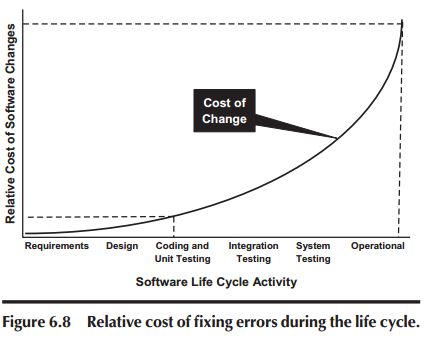
\includegraphics[width=0.5\textwidth]{p2}
\end{figure}\\
\textbf{6.5.2 Software Peer Review Process}\\
The SDP, or the Peer Review Plan if there is one, must defne
the processes to be followed for each type of Peer Review to
be used on each of the software work products and for each
software category (categories are described in Section 1.8).
The process should include preparing for the Peer Review,
conducting the Peer Reviews, and analyzing the resulting
Peer Review data. The planning for Peer Reviews is part of
the software development planning process. The evaluation
criteria for each software product must be supplied to the
Peer Review participants. Figure 6.9 is an example overview
of a typical Software Peer Review Process.
System Critical software (whether deliverable or nondeliverable) must undergo the most formal, robust Peer
Review process for their initial development and for signifcant changes. Support software and minor changes to software work products may undergo a less formal Peer Review.\\
\textbf{6.5.3 Preparing for Software Peer Reviews}\\
A software project typically adopts the standard Peer Review
process of its parent organization for conducting Software
Peer Reviews. SPR preparation should consist of entry/exit
criteria, defnition of the steps, and roles with appropriate participants identifed. Peer reviews must be scheduled, planned,
and tracked by the subsystem and/or SwIPT leads in order to:\\
Determine what type of Peer Review will be conducted
on each work product.
- Identify key reviewers who must participate in each
Peer Review plus invited reviewers.
- Ensure that each software work product satisfes the
Peer Review entry criteria.
- Ensure all reviewers understand their roles in the Peer
Review.
- Confrm that the participants have reviewed each work
product prior to the Peer Review, using the predetermined review checklist for that product.
A subsystem (or lower level) Software Peer Review Plan
should be prepared to defne the procedures, data collection and reporting for Peer Reviews and product evaluations. Te
implementation of the SPR Plan is the responsibility of the
subsystem/element SwIPT software personnel Lead. The SPR
Plan typically defnes the types of Peer Reviews to be held.
Peer reviews should have varying levels of formality, ranging
from Formal Inspections to Colleague Reviews and maybe
some in between:\\
- Formal Inspections: Formal inspections are performed
to verify that software products conform to established
technical decisions and applicable standards and procedures. Formal Inspections are the most thorough
Peer Review and are conducted initially when the
product has reached enough maturity and completeness for a thorough review or when extensive changes
are involved. The Software Lead should review all the
changes and determine if additional Peer Reviews need
to be held.\\
- Colleague Reviews: Tis is the least formal type of
review used primarily to review portions of a System
Critical work product during its development to
improve the quality of the product during its development. A Colleague Review can be conducted by one
person, and it may be used for relatively minor updates
to software products that have already undergone a
Formal Inspection. Colleague Reviews are not a substitute for required inspections.\\
\textbf{6.5.4 Conducting Software Peer Reviews}\\
Software Peer Reviews must be ongoing during the development tasks, prior to work products being released to subsequent activities. The SDP should include a table similar
to example Table 6.9 showing the set of development work
products that normally require Peer Reviews. The goal of
each Peer Review is to identify work product defects as early
as possible in the lifecycle. Defects identifed and corrected
early always results in a lower cost to resolve than fnding and
fxing them later.\\
\textbf{Peer Review Roles.} The typical roles include a moderator, reviewers, monitor /coordinator, recorder and the Product
Developer or Document Author. Inspection training or skills from past experience should be required for all participants. 
\begin{figure}[h!]
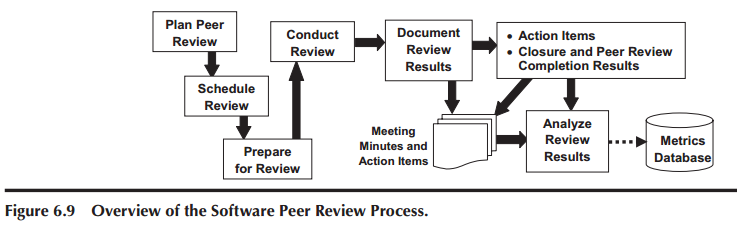
\includegraphics[width=0.5\textwidth]{p3}
\end{figure} 
\begin{figure}[h!]
	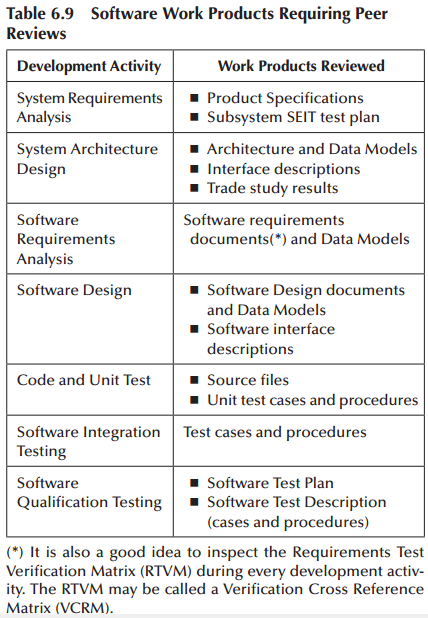
\includegraphics[width=0.5\textwidth]{last}
\end{figure} 
 
The following is a brief description of each key role:\\
- The Peer Review moderator is instrumental in setting up the inspection, and ensuring the key reviewers
for the work product are present and prepared for the
inspection.\\
- Reviewers should be trained to perform various inspection roles. Tese trained inspectors participate to identify defects, improvements and issues in the product(s)
being examined and contribute to the determination
of the product’s ability to proceed to the next development activity.\\
- The Monitor/Coordinator ensures the Peer Review
process is held in accordance with the approved tailored Peer Review process, and they are tasked to compile and analyze Peer Review metrics, maintain a list of
qualifed inspectors, and oversee the implementation
of continuous process improvement within the Peer
Review process.\\
- The Recorder is responsible for creating Peer Review
records in hard copy or electronic fles.
\textbf{The Peer Review Package.} A Peer Review announcement and review package should be distributed about a week
prior to the Peer Review. Participants must review the work
product against higher-level requirements, using checklists
aimed at fnding major system problems and for compliance with templates, standards, and guidelines. Findings
must be documented, assigned to responsible individuals as
action items for resolution by a due date, and then tracked
to closure.\\
\textbf{6.5.5 Analyzing Software Peer Review Data}\\
The metrics collected during Peer Reviews can be used to
provide visibility into the quality of the produced documents
and code, the effectiveness of the SPR, and to indicate the
need for corrective or process changes. At the end of each
development activity, participating organizations analyze the
root causes of defciencies to identify process improvements
that can be implemented to avoid future occurrence of those
defciencies.
\textbf{Defect Data.} The number of defects expected from a
Peer Review depends on when in the life cycle the review
is conducted. Table 6.10 is an example of a defect removal
scenario showing the incremental burn down of 300
defects injected during coding to seven defects during feld
testing.
Analysis of historical SPR data can provide many benefts such as setting expectations for the Peer Reviews conducted on requirements, design, coding, and test products.
For software, code count and complexity can be used, as well
as experience from prior programs, to predict the number of
defects from each life cycle activity. In fact, fxing defects is
one of the largest variables in estimating project cost.
A Defect Prevention Team can compare predicted versus
actual defects to assess the quality of the product at the end
of each activity. Tey can analyze the defect causes to initiate defect prevention process improvements for subsequent
builds. Required defect data and associated metrics for Peer
Reviews should be described in the Software Measurement
Plan. See Subsection 3.9.8 for defect estimation.
\textbf{Peer Review Data.} Typical Peer Review data that
should be collected at each review and analyzed for potential
improvement of the Peer Review process include:
- Identifcation of the work product(s) under review\\
- Meeting date, time, location and completion date\\
- Number of attendees and preparation time spent by
each reviewer\\
- Size of the work product(s) reviewed\\
- Inspection type and role assignments\\
- Peer Review Defect List\\
- Amount of time spent in rework of the software work
product and to close action items

\end{document}